% le design de chaque page
Le design de chaque page a été faite selon les critères donnés par le responsable de l'unité. Il fallait donc reprendre le zoning de page déjà existante :
\begin{itemize}
    \item "Accueil" : https://www.louvre.fr/
    \item "Actualité" : https://www.lesechos.fr/
    \item "Logement" : https://www.seloger.com/
    \item "Voyage" : https://sejour.govoyages.com/
\end{itemize}
\vspace{2\baselineskip}


\begin{minipage}{0.5 \linewidth}
    \hspace{-3cm}
    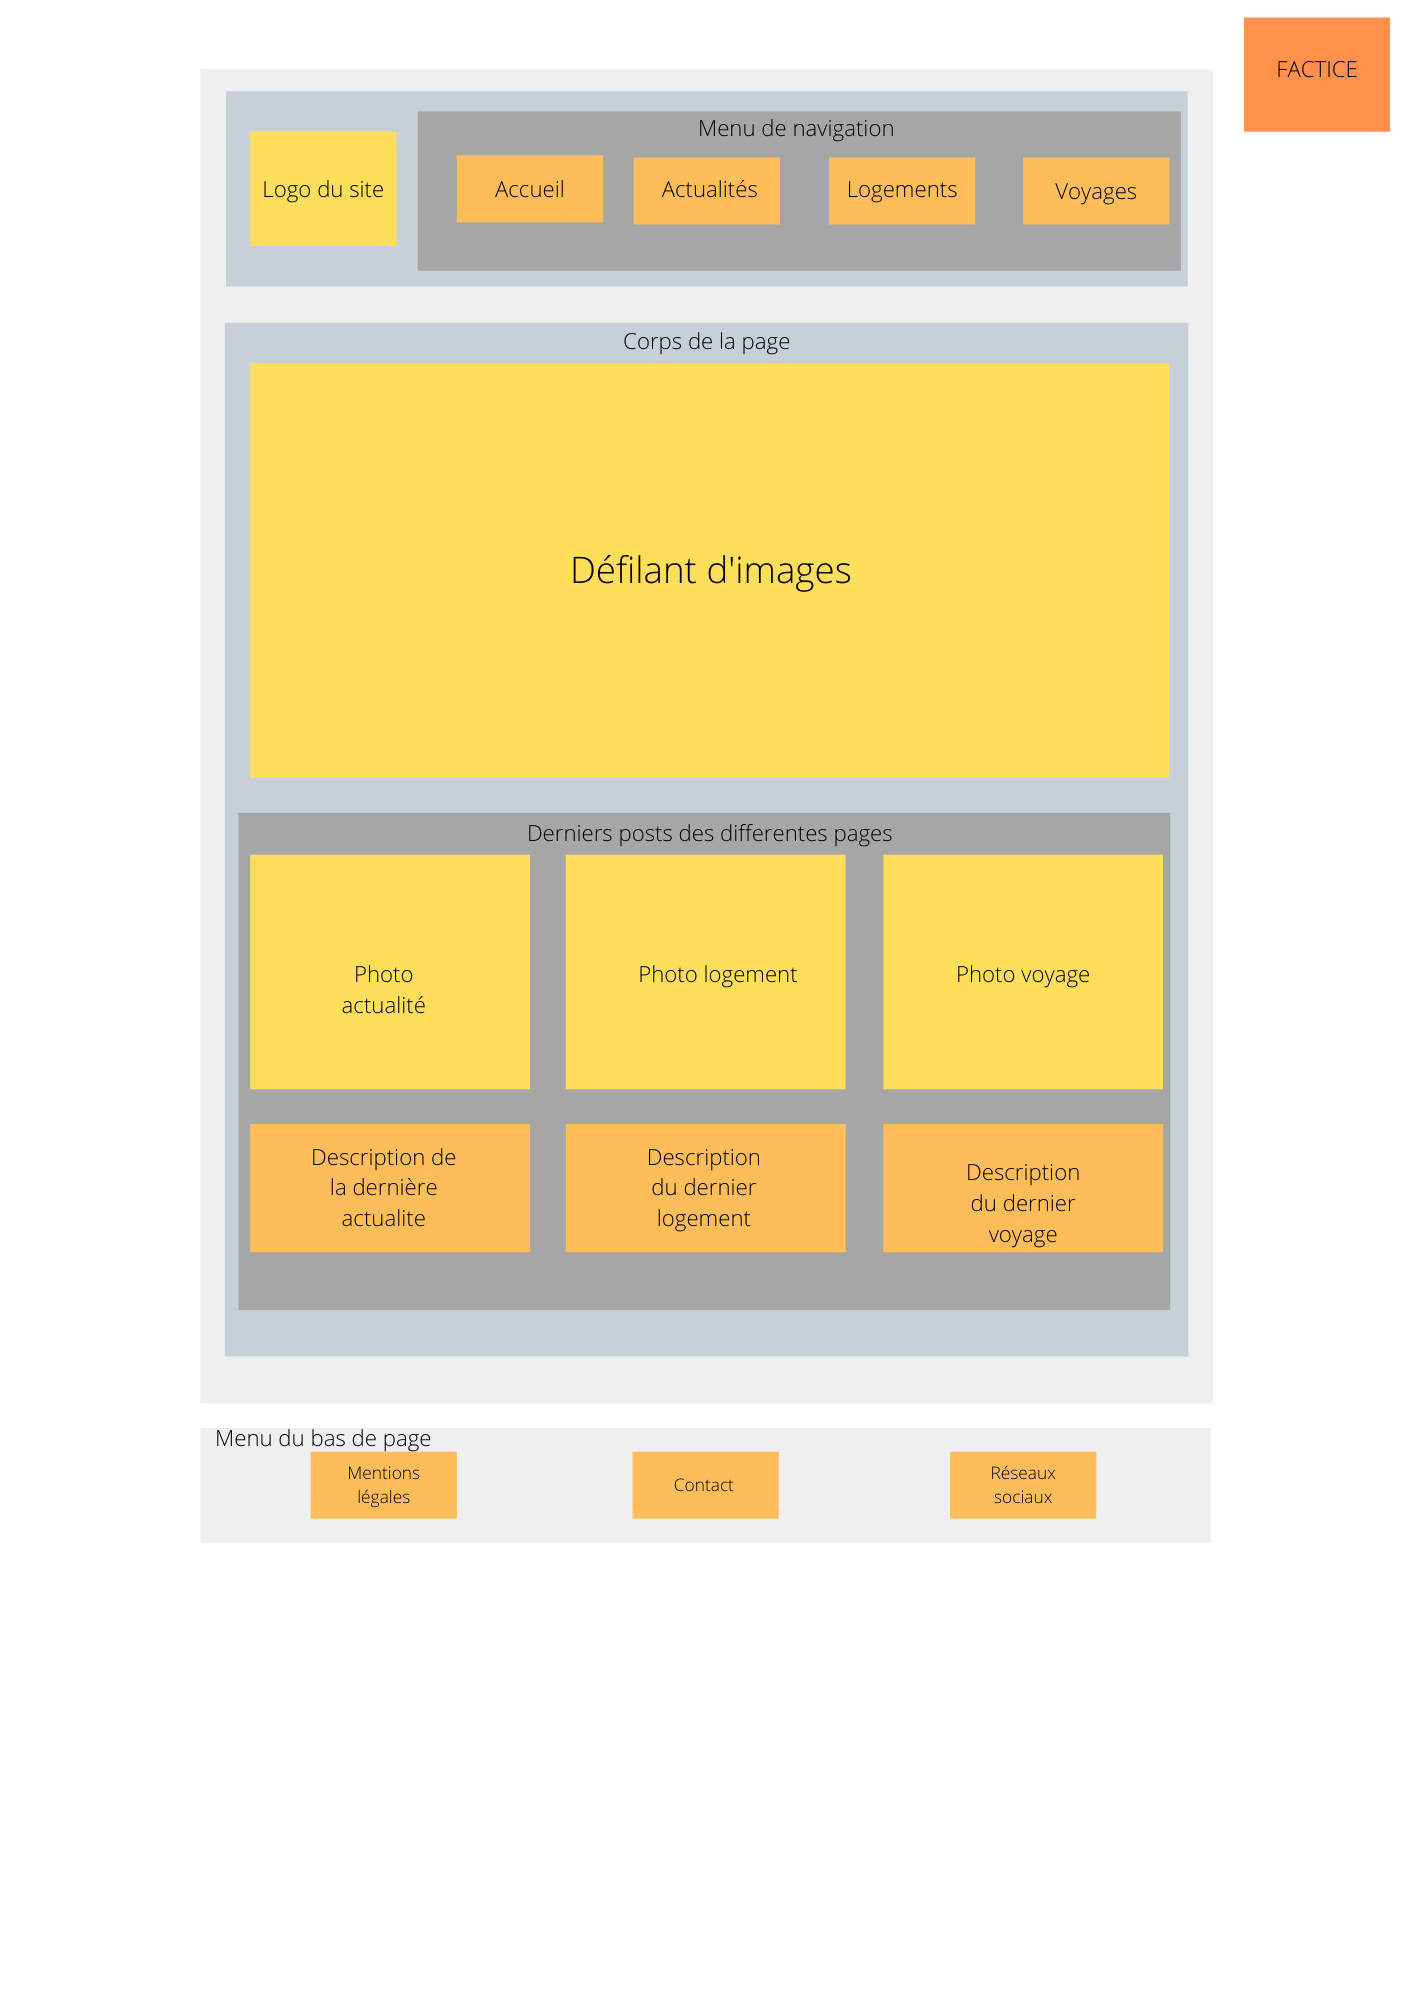
\includegraphics[scale=0.3]{accueil.png}
\end{minipage} \hfill
\begin{minipage}{0.5 \linewidth}
    Cette page "accueil" contient le menu en haut de page qui est commun avec les autres pages, ainsi que le pied de page, lui aussi commun avec l'intégralité des pages du projet. 
    On retrouve aussi un défilant de 4 images dans la partie supérieure du corps de la page. 
    En dessus, 3 actualités en lien avec les différentes pages sont composées d'une description et d'une image.
\end{minipage}

\begin{minipage}{0.5 \linewidth}
   Cette page "actualité" contient, comme précédemment, le menu en haut de page et le bas de page. 
   Elle a sa dernière actualité en plus grande pour la mettre en avant : iframe d'une carte intergalactique avec la description de l'actualité. 
   Deux autres sont ajoutées à la suite, les images sont plus petites et les descriptions plus concises.
\end{minipage} \hfill
\begin{minipage}{0.5 \linewidth}
    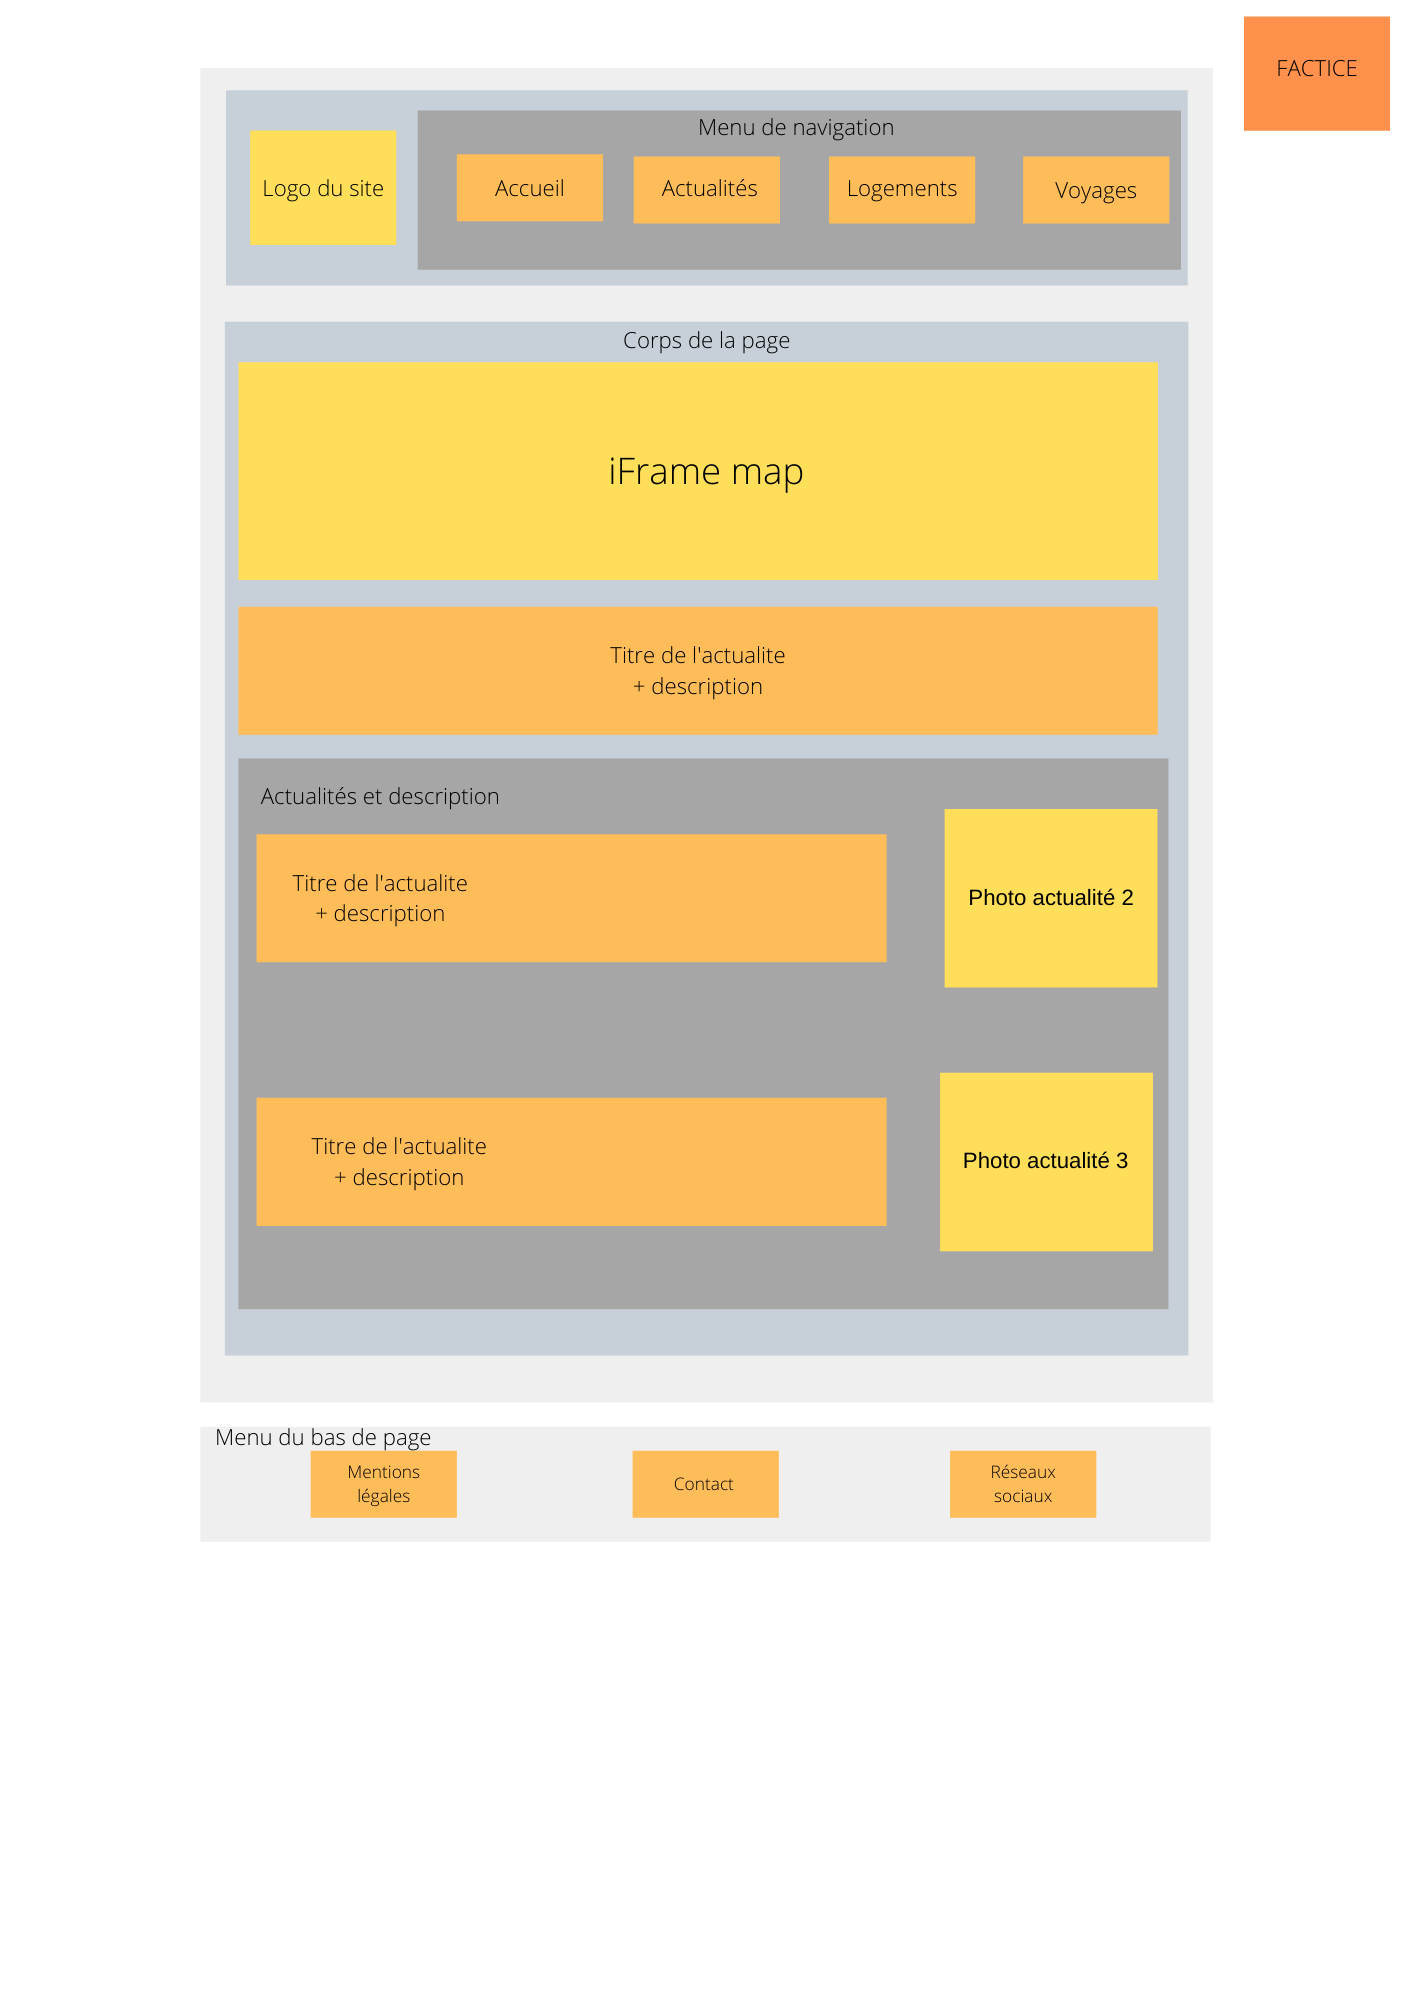
\includegraphics[scale=0.21]{actualite.png}
\end{minipage}

\begin{minipage}{0.5 \linewidth}
    \hspace{-1cm}
    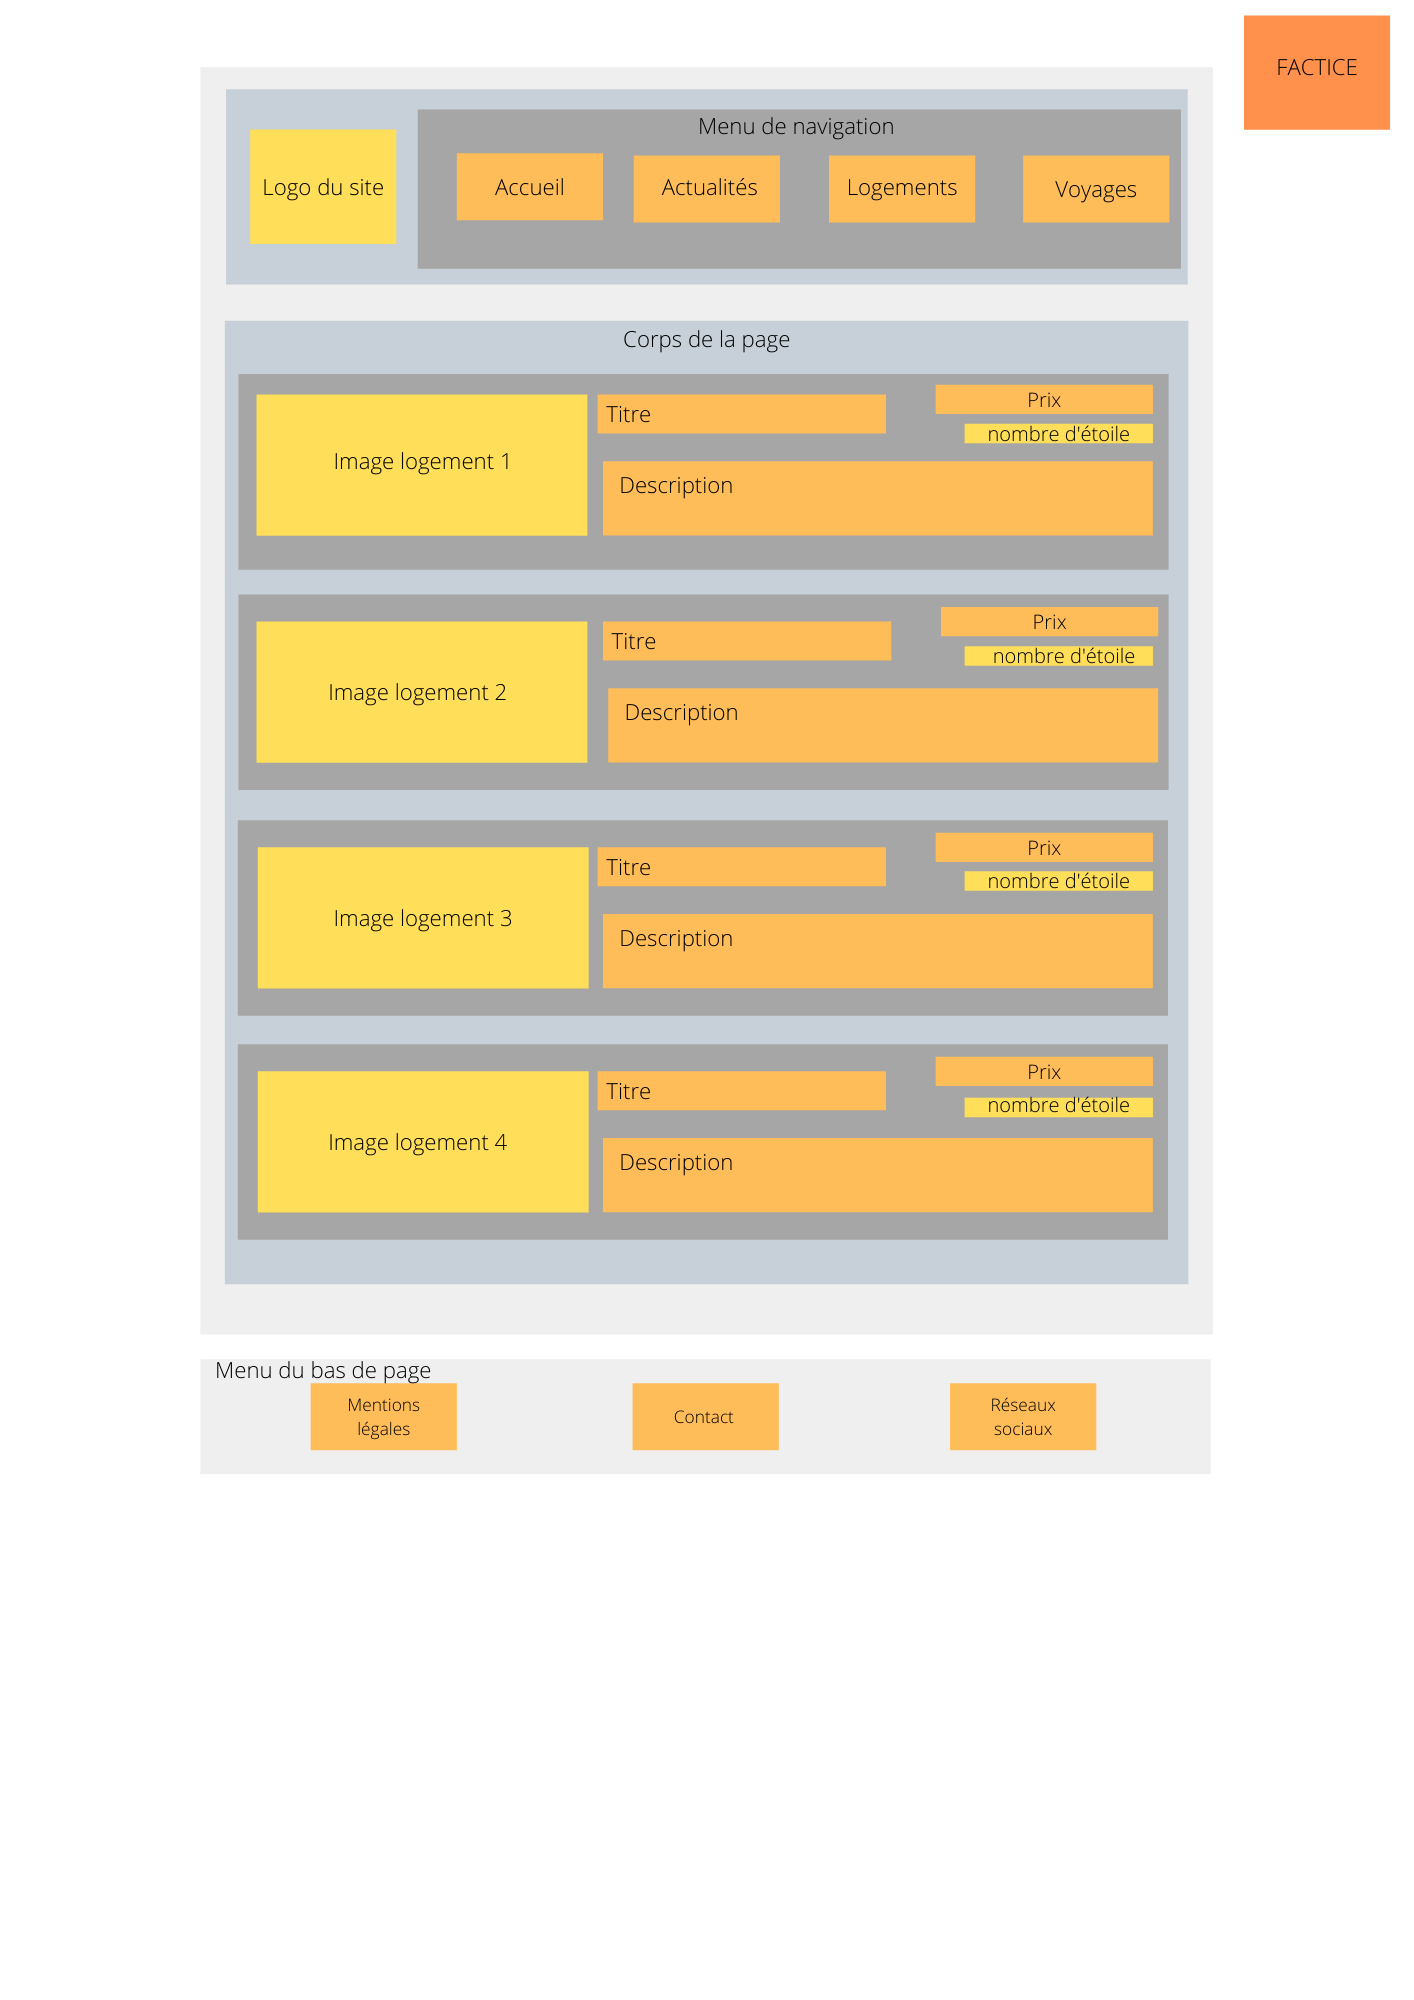
\includegraphics[scale=0.21]{logement.png}
\end{minipage} \hfill
\begin{minipage}{0.5 \linewidth}
    De même pour la page "logement", le menu en haut et bas de page sont disponibles.
    Ici, il y a quatre types de logement possible. 
    Ils sont tous implémenté de la même façon : image d'illustration à gauche, le titre du voyage et sa description, le prix ainsi que la note attribuée au logement par les précèdent clients.
\end{minipage}

\begin{minipage}{0.3 \linewidth}
    Pour finir, la page "voyage" a elle aussi les menus du haut et du bas de page.
    La structure est différentes pour celle-ci : il y a six voyages disponibles.
    Ils sont organisés sur deux lignes.
    Chacun à une image, un titre et une description ainsi qu'un prix.
\end{minipage} \hfill
\begin{minipage}{0.5 \linewidth}
    \hspace{-2cm}
    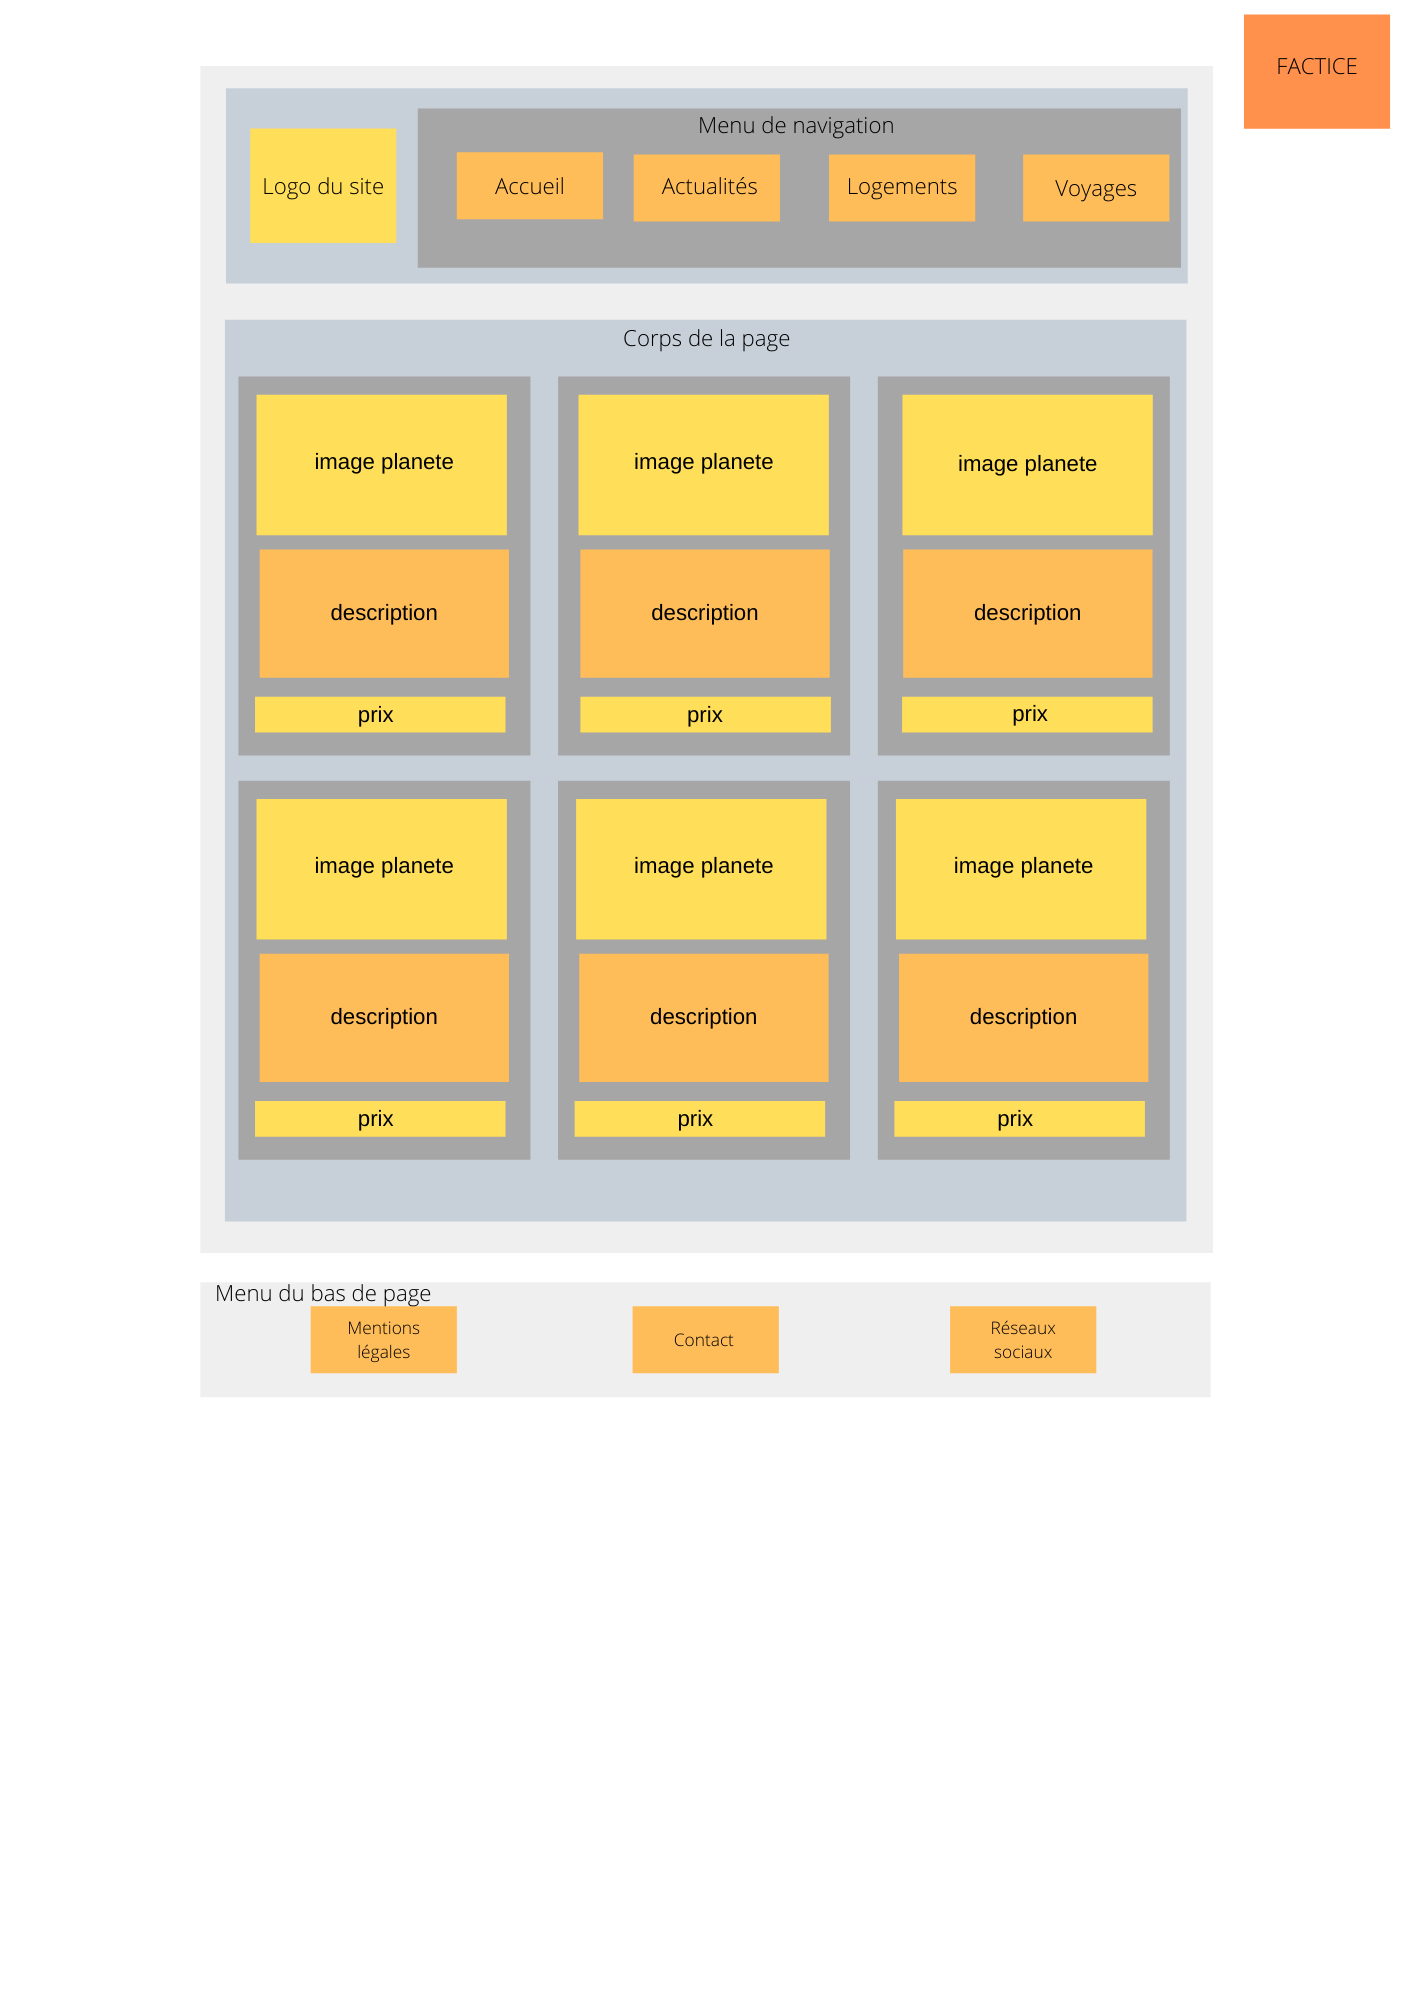
\includegraphics[scale=0.3]{voyage.png}
\end{minipage}

Sur les pages "logements" et "voyages", nous avons implémenté un tableau de conversion des monnaies galactiques. 
Celui-ci peut disparaître hors de la page ou apparaître sur le côté par le simple survole des flèches à cet effet.

Les pages "mention légale", "contact", "réseaux sociaux" n'ont pas été faite sur un modèle. 
Les groupes étaient libres pour le zooning de celles-ci. 

\newpage